\documentclass[aspectratio=169, table, 12pt]{beamer}

% Preamble bersama seluruh slide mata kuliah ini.
% Dipanggil dari slides/sessionXX/sessionXX.tex tepat sesudah baris
% \documentclass[aspectratio=169, table, 12pt]{beamer}
% Paket tambahan yang hanya dibutuhkan satu sesi ditulis di berkas sesi itu.

\usepackage{colortbl}
\usepackage{xcolor}
\usepackage{listings}
\usepackage{tabularx}
\usepackage{booktabs}
\usepackage{tikz}
\usepackage{pgfplots}
\pgfplotsset{compat=1.18}
\usetikzlibrary{arrows.meta, positioning, calc, fit, shapes.geometric,
	shapes.multipart, backgrounds, matrix, chains, trees}

\makeatletter
\def\input@path{{../theme/}}
\makeatother
\graphicspath{{../theme/}{../../figures/}}
\usetheme{Pradita}

\definecolor{praditagreen}{RGB}{37, 113, 71}

% Tema membuat garis tabel berwarna putih. Dikembalikan agar tabel terbaca.
\arrayrulecolor{black}
\setlength{\arrayrulewidth}{0.5pt}

\lstdefinelanguage{yaml}{
	basicstyle=\ttfamily\scriptsize,
	keywordstyle=\color{blue}\bfseries,
	commentstyle=\color{gray}\itshape,
	stringstyle=\color{red},
	showstringspaces=false,
	breaklines=true,
	frame=lines,
	numbers=none,
	backgroundcolor=\color{lightgray!10},
	tabsize=2,
	morecomment=[l]{\#}
}

\lstdefinelanguage{json}{
	basicstyle=\ttfamily\scriptsize,
	stringstyle=\color{red},
	commentstyle=\color{gray},
	breaklines=true,
	showstringspaces=false,
	tabsize=2,
	numbers=none,
	frame=lines,
	backgroundcolor=\color{lightgray!10},
	string=[s]{"}{"}
}

\lstdefinelanguage{bash}{
	keywords={},
	basicstyle=\ttfamily\scriptsize,
	ndkeywords={docker, kubectl, helm, curl, git, terraform},
	ndkeywordstyle=\color{purple}\bfseries,
	sensitive=true,
	commentstyle=\color{gray},
	numbers=none,
	breaklines=true,
	frame=lines,
	backgroundcolor=\color{lightgray!10},
	tabsize=2,
	comment=[l]{\#},
	showstringspaces=false
}

\lstdefinelanguage{http}{
	keywords={GET, POST, PUT, PATCH, DELETE, HEAD, OPTIONS, HTTP},
	basicstyle=\ttfamily\scriptsize,
	keywordstyle=\color{blue}\bfseries,
	sensitive=true,
	numbers=none,
	breaklines=true,
	frame=lines,
	backgroundcolor=\color{lightgray!10},
	tabsize=2,
	showstringspaces=false
}

\subtitle{IT40713 · Cloud-Native \& Microservices Architecture}
\author{\textbf{Alfa Yohannis}}


\title{\Huge Data Microservices:\\ \vspace{10pt} Saga dan Outbox}

\begin{document}

\frame{\titlepage}

\begin{frame}
  \frametitle{Isi Pertemuan}
  \vspace{14pt}
  \begin{columns}[t]
    \column{0.5\textwidth}
    {\small\tableofcontents[sections={1-4}]}

    \column{0.5\textwidth}
    {\small\tableofcontents[sections={5-8}]}
  \end{columns}
\end{frame}

\begin{frame}{\hfill}
  \centering
  \Huge{\textbf{Mengapa memecah sistem\\justru bisa membuat\\data pasien makin kacau?}}
\end{frame}

\section{Tujuan dan Konteks}

\begin{frame}{\hfill}
  \centering
  \Huge{\textbf{Tujuan dan Konteks}}
\end{frame}

\begin{frame}{{\Large Tujuan Pembelajaran}}
  \vspace{10pt}
  \begin{itemize}
    \item Menjelaskan alasan setiap layanan memiliki datanya sendiri dan risiko
          basis data bersama.
    \item Merancang saga beserta langkah kompensasinya untuk satu proses
          lintas layanan.
    \item Menjelaskan cara pola \textit{transactional outbox} mencegah data dan
          \textit{event} tidak sinkron.
  \end{itemize}
\end{frame}

\begin{frame}{{\Large Data Pasien Medikara Health yang Tersebar}}
  \vspace{6pt}
  \small
  \begin{itemize}
    \item Satu pasien di rumah sakit Bekasi dan Depok punya dua nomor rekam
          medis.
    \item Alamat baru di Medikara+ tidak sampai ke SIMRS Bekasi.
    \item Laporan kunjungan keuangan dan pelayanan tidak pernah sama.
    \item Layanan baru yang tetap menulis ke basis data SIMRS hanya memindahkan
          ketergantungan.
    \item Tiga pertanyaan: siapa pemilik data, bagaimana proses lintas layanan
          tetap utuh, bagaimana laporan tetap tersedia?
  \end{itemize}
\end{frame}

\IfFileExists{../../figures/ch10-diagram-konsep.png}{%
\begin{frame}{{\Large Diagram Konsep Bab 10}}
  \centering
  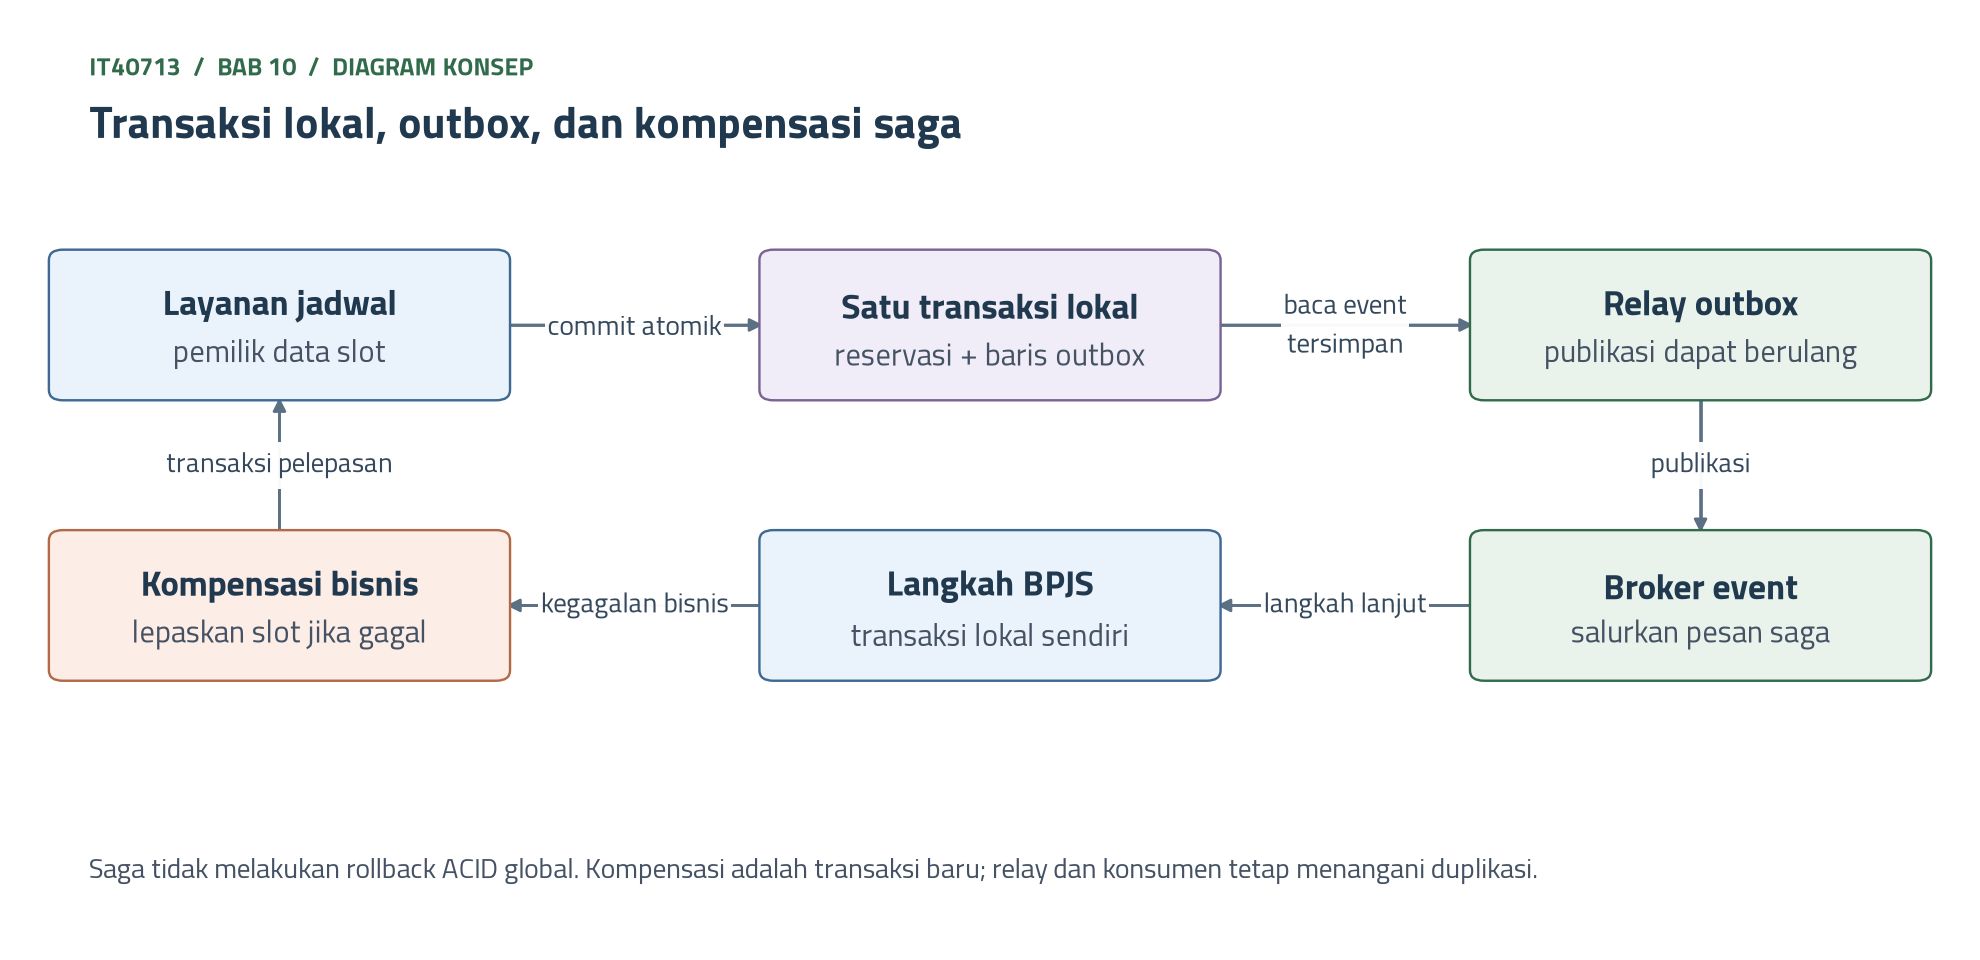
\includegraphics[width=0.96\textwidth,height=0.77\textheight,keepaspectratio]{../../figures/ch10-diagram-konsep.png}
\end{frame}
}{}

\section{Database per Service}

\begin{frame}{\hfill}
  \centering
  \Huge{\textbf{Database per Service}}
\end{frame}

\begin{frame}{{\Large Database per Service dan Basis Data Bersama}}
  \vspace{6pt}
  \small
  \begin{itemize}
    \item Data setiap layanan privat, hanya diakses lewat API miliknya.
    \item Basis data bersama: beberapa modul menulis tabel yang sama,
          sebuah \textit{anti-pattern}.
    \item Privat tidak berarti server sendiri: tabel privat, skema privat, atau
          server per layanan.
    \item Harga: transaksi dan \textit{query} lintas layanan menjadi sulit.
  \end{itemize}
  \vspace{6pt}
  {\small Analogi: buku besar di meja tengah yang ditulisi semua bagian,
  dibandingkan lemari arsip per bagian dengan loket salinan.}
\end{frame}

\begin{frame}{{\Large Dua Susunan Data}}
  \centering
  \eadiagram{../../figures/ch10-basis-data-bersama.tex}
\end{frame}

\begin{frame}{{\Large Dampak bagi Organisasi}}
  \footnotesize
  \begin{tabularx}{\textwidth}{>{\raggedright\arraybackslash}p{2.8cm}
      >{\raggedright\arraybackslash}X >{\raggedright\arraybackslash}X}
    \hline
    \textbf{Aspek} & \textbf{Basis data bersama} &
      \textbf{\textit{Database per service}} \\
    \hline
    Perubahan struktur & Disepakati semua tim pengguna & Diputuskan tim
      pemilik; kontrak dijaga \\
    \hline
    Kepemilikan data & Kabur & Satu pemilik per data \\
    \hline
    Beban dan kegagalan & \textit{Query} berat memperlambat semua modul &
      Terkurung di satu layanan \\
    \hline
    Kontrol akses & Banyak akun punya hak tulis & Lewat API yang dicatat \\
    \hline
    Harga & Rendah di awal & Transaksi dan \textit{query} lintas layanan perlu
      pola khusus \\
    \hline
  \end{tabularx}
\end{frame}

\begin{frame}{{\Large Tiga Cara Memperoleh Data Milik Layanan Lain}}
  \footnotesize
  \begin{tabularx}{\textwidth}{>{\raggedright\arraybackslash}p{3.2cm}
      >{\raggedright\arraybackslash}X >{\raggedright\arraybackslash}X}
    \hline
    \textbf{Cara} & \textbf{Kelebihan} & \textbf{Harga} \\
    \hline
    Memanggil API pemilik & Data selalu terbaru & Ikut terganggu bila pemilik
      tidak tersedia \\
    \hline
    Salinan lokal dari \textit{event} & Tetap berjalan walaupun pemilik mati &
      Bisa tertinggal beberapa saat \\
    \hline
    \textit{Read model} khusus & Cepat untuk laporan lintas layanan & Komponen
      tambahan, batas kesegaran \\
    \hline
  \end{tabularx}

  \vspace{10pt}
  \small
  Aturan bersama: salinan tidak pernah diubah oleh pembacanya.
\end{frame}

\begin{frame}{{\Large Kasus Medikara: Satu Tabel Pasien, Tiga Penulis}}
  \vspace{6pt}
  \small
  \begin{itemize}
    \item Tabel pasien SIMRS Bekasi: 64 kolom; pendaftaran 31, keuangan 14,
          laboratorium 9, tanpa pemilik 10.
    \item 23 akun punya hak tulis, termasuk satu akun vendor laboratorium.
    \item Kolom nomor kartu penjamin diperlebar: pendaftaran gagal 3 jam, 410
          pasien didaftarkan dengan kertas.
    \item Usulan: Layanan Identitas Pasien, Layanan Penjaminan, dan Layanan
          Rekam Medis menjadi pemilik.
    \item Dipindah bertahap dengan pola \textit{strangler fig} (Bab 14).
  \end{itemize}
\end{frame}

\section{Transaksi Terdistribusi}

\begin{frame}{\hfill}
  \centering
  \Huge{\textbf{Transaksi Terdistribusi}}
\end{frame}

\begin{frame}{{\Large Batas Two-Phase Commit}}
  \vspace{6pt}
  \small
  \begin{itemize}
    \item Sifat ACID kini hanya berlaku di dalam satu layanan.
    \item 2PC: koordinator bertanya "siap?", lalu semua peserta menyimpan atau
          semua membatalkan.
    \item Semua peserta harus tersedia: 4 layanan 99,5 persen menjadi sekitar
          98,0 persen.
    \item Waktu tidak tersedia per bulan naik dari 3,6 jam menjadi sekitar 14,3
          jam.
    \item Kunci data tertahan; \textit{broker}, BPJS Kesehatan, dan SATUSEHAT
          tidak dapat ikut.
  \end{itemize}
\end{frame}

\begin{frame}{{\Large Eventual Consistency}}
  \vspace{6pt}
  \small
  \begin{itemize}
    \item Bila tidak ada perubahan baru, semua pembaca akhirnya melihat nilai
          yang sama.
    \item Jendela ketidakkonsistenan: rentang sampai semua pembaca melihat nilai
          baru (Vogels, 2009).
    \item Analogi: transfer antarbank, "transaksi sedang diproses".
    \item Tiga pertanyaan bagi pengguna bisnis: berapa lama selisih diterima,
          apa yang terlihat, apa yang terjadi bila gagal?
  \end{itemize}
\end{frame}

\begin{frame}{{\Large Toleransi Selisih pada Lima Data Medikara}}
  \footnotesize
  \begin{tabularx}{\textwidth}{>{\raggedright\arraybackslash}p{3.6cm}
      >{\raggedright\arraybackslash}p{2.6cm} >{\raggedright\arraybackslash}X}
    \hline
    \textbf{Data} & \textbf{Selisih diterima} & \textbf{Pendekatan} \\
    \hline
    Slot jadwal dokter & Tidak ada & Dikunci di Layanan Jadwal \\
    \hline
    Stok obat apotek & Detik & Stok dipesan di layanan pemilik \\
    \hline
    Status kepesertaan & Menit & Status "menunggu verifikasi" \\
    \hline
    Hasil laboratorium di Medikara+ & 5 menit & Pemberitahuan saat tersedia \\
    \hline
    Laporan kunjungan harian & Beberapa jam & \textit{Read model} dari
      \textit{event} \\
    \hline
  \end{tabularx}

  \vspace{8pt}
  \small
  Selisih hanya diterima di antara layanan, bukan di dalam satu layanan.
\end{frame}

\section{Saga dan Kompensasi}

\begin{frame}{\hfill}
  \centering
  \Huge{\textbf{Saga dan Kompensasi}}
\end{frame}

\begin{frame}{{\Large Gagasan Saga}}
  \vspace{6pt}
  \small
  \begin{itemize}
    \item Garcia-Molina dan Salem (1987): transaksi panjang dipecah menjadi
          $T_1, \ldots, T_n$.
    \item Setiap $T_i$ punya kompensasi $C_i$ yang membalik akibat bisnisnya.
    \item Hasil: semua $T$ selesai, atau $T_1 \ldots T_j$ lalu $C_j \ldots C_1$.
    \item Richardson: rangkaian transaksi lokal di beberapa layanan.
  \end{itemize}
  \vspace{6pt}
  {\small Analogi: perjalanan dinas. Hotel penuh, tiket pesawat dibatalkan
  dengan pengembalian dana, dan keduanya tercatat.}
\end{frame}

\begin{frame}{{\Large Saga Pendaftaran Pasien Rujukan}}
  \centering
  \eadiagram{../../figures/ch10-saga-rujukan.tex}
\end{frame}

\begin{frame}{{\Large Kompensasi Bukan Rollback}}
  \vspace{6pt}
  \small
  \begin{itemize}
    \item Kompensasi adalah transaksi baru; pesan terkirim dikompensasi dengan
          pesan ralat.
    \item Tidak selalu batal: tawarkan jalur pembayaran umum sebelum jadwal
          dilepas.
    \item Dapat dikompensasi, titik penentu (\textit{pivot}), dan dapat diulang
          (\textit{retriable}).
    \item Langkah yang tidak dapat dibatalkan diletakkan dekat titik penentu.
    \item Saga tidak punya isolasi: kunci semantik
          \texttt{MENUNGGU\_VERIFIKASI}.
  \end{itemize}
\end{frame}

\begin{frame}{{\Large Choreography dan Orchestration pada Saga}}
  \footnotesize
  \begin{tabularx}{\textwidth}{>{\raggedright\arraybackslash}p{3.2cm}
      >{\raggedright\arraybackslash}X >{\raggedright\arraybackslash}X}
    \hline
    \textbf{Aspek} & \textbf{\textit{Choreography}} &
      \textbf{\textit{Orchestration}} \\
    \hline
    Pengatur alur & Tersebar di setiap layanan & Satu pengatur saga \\
    \hline
    Melacak status & Sulit, disusun dari banyak \textit{event} & Mudah,
      tercatat di pengatur \\
    \hline
    Risiko & Ketergantungan melingkar tak terlihat & Logika menumpuk di
      pengatur \\
    \hline
    Cocok untuk & Saga pendek, dua sampai tiga langkah & Saga panjang, perlu
      jejak audit \\
    \hline
  \end{tabularx}

  \vspace{8pt}
  \small
  Pembatalan janji temu: \textit{choreography}. Pendaftaran rujukan:
  \textit{orchestration}.
\end{frame}

\begin{frame}{{\Large Kasus Medikara: Saga Rujukan}}
  \vspace{6pt}
  \small
  \begin{itemize}
    \item Sekitar 3.600 rujukan per bulan; 4 persen, atau 144, gagal verifikasi
          BPJS Kesehatan.
    \item Kini slot dilepas rata-rata dua hari kemudian: sekitar 36 jam praktik
          spesialis per bulan terkunci.
    \item Saga \textit{orchestration} dengan pengatur di Layanan Rujukan.
    \item Aturan bisnis: dua jam kerja untuk menawarkan jalur lain sebelum C3.
    \item Kompensasi T2 melepas tautan rujukan; identitas pasien tetap.
  \end{itemize}
\end{frame}

\section{Transactional Outbox}

\begin{frame}{\hfill}
  \centering
  \Huge{\textbf{Transactional Outbox}}
\end{frame}

\begin{frame}{{\Large Masalah Dual Write}}
  \footnotesize
  \begin{tabularx}{\textwidth}{>{\raggedright\arraybackslash}p{3.6cm}
      >{\raggedright\arraybackslash}X >{\raggedright\arraybackslash}X}
    \hline
    \textbf{Urutan} & \textbf{Keadaan setelah gagal} & \textbf{Akibat bisnis} \\
    \hline
    Simpan data, lalu terbitkan \textit{event} & Slot terkunci, \textit{event}
      hilang & Saga macet \\
    \hline
    Terbitkan \textit{event}, lalu simpan data & \textit{Event} terbit,
      penyimpanan batal & Kabar jadwal palsu \\
    \hline
    \textit{Transactional outbox} & Tersimpan atau batal bersama &
      \textit{Event} pasti terbit, mungkin dua kali \\
    \hline
  \end{tabularx}

  \vspace{10pt}
  \small
  Analogi: baki surat keluar. Kurir datang berkala, mengantar, lalu mencentang
  buku ekspedisi.
\end{frame}

\begin{frame}{{\Large Alur Transactional Outbox}}
  \centering
  \eadiagram{../../figures/ch10-outbox.tex}
\end{frame}

\begin{frame}{{\Large Penerbit dan Consumer yang Idempoten}}
  \vspace{6pt}
  \small
  \begin{itemize}
    \item \textit{Polling publisher}: \textit{query} berkala, mudah dimulai.
    \item \textit{Transaction log tailing} dengan CDC: hampir seketika, perlu
          perangkat khusus.
    \item Jaminan \textit{at-least-once}: \textit{consumer} menolak nomor
          \textit{event} yang sudah diproses.
    \item Medikara+: 28.000 janji temu per bulan; 0,3 persen \textit{event}
          hilang berarti 84 pasien tanpa pengingat.
    \item \texttt{TagihanTerbit} kembar ke ERP: dua piutang untuk satu
          kunjungan.
  \end{itemize}
\end{frame}

\section{CQRS dan Read Model}

\begin{frame}{\hfill}
  \centering
  \Huge{\textbf{CQRS dan Read Model}}
\end{frame}

\begin{frame}{{\Large CQRS dan Read Model}}
  \vspace{6pt}
  \small
  \begin{itemize}
    \item Model untuk mengubah data dipisah dari model untuk membaca data.
    \item \textit{Read model} dibangun dari \textit{event} layanan pemilik.
    \item Manfaat: layanan operasional tidak terbebani, laporan lintas layanan,
          dapat dibangun ulang.
    \item Batas: tertinggal detik sampai menit; slot jadwal tetap dicek di
          pemiliknya.
    \item Fowler: bagi sebagian besar sistem, CQRS menambah kerumitan berisiko.
  \end{itemize}
  \vspace{4pt}
  {\small Analogi: papan keberangkatan di bandara.}
\end{frame}

\begin{frame}{{\Large Read Model untuk Laporan}}
  \centering
  \eadiagram{../../figures/ch10-read-model.tex}
\end{frame}

\begin{frame}{{\Large Kasus Medikara: Laporan Spreadsheet}}
  \vspace{6pt}
  \small
  \begin{itemize}
    \item 14 laporan bulanan; 6 staf selama 3 hari kerja, sekitar 144 jam kerja.
    \item Jumlah kunjungan antarlaporan berbeda sampai 3 persen.
    \item Empat laporan pertama: kunjungan harian, pendapatan per penjamin,
          waktu tunggu rujukan, status klaim.
    \item Definisi "kunjungan" disepakati sekali dalam aturan proyeksi.
    \item Dua bulan berjalan berdampingan sebelum \textit{spreadsheet}
          dihentikan.
  \end{itemize}
\end{frame}

\section{Data Pasien}

\begin{frame}{\hfill}
  \centering
  \Huge{\textbf{Satu Pasien,\\Satu Rekam Medis}}
\end{frame}

\begin{frame}{{\Large Identitas Pasien Induk dan Persetujuan}}
  \vspace{6pt}
  \small
  \begin{itemize}
    \item Layanan Identitas Pasien menjalankan indeks pasien induk (MPI).
    \item Catatan ganda ditautkan, bukan dihapus; FHIR \texttt{Patient.link}.
    \item UU PDP: data kesehatan adalah data pribadi spesifik.
    \item Layanan Persetujuan menjadi pemilik catatan persetujuan pasien.
    \item \textit{Event} membawa data seperlunya; rincian dibaca lewat API.
  \end{itemize}
  \vspace{4pt}
  {\small Analogi: nomor induk mahasiswa yang dipakai semua unit kampus.}
\end{frame}

\begin{frame}{{\Large Contoh Peta Kepemilikan Data}}
  \footnotesize
  \begin{tabularx}{\textwidth}{>{\raggedright\arraybackslash}p{3.4cm}
      >{\raggedright\arraybackslash}p{2.6cm} >{\raggedright\arraybackslash}X}
    \hline
    \textbf{Entitas data} & \textbf{Pemilik} & \textbf{Cara memperoleh} \\
    \hline
    Identitas pasien induk & Identitas Pasien & API pencarian;
      \texttt{PasienDiperbarui} \\
    \hline
    Persetujuan pasien & Persetujuan & API wajib diperiksa \\
    \hline
    Rujukan & Rujukan & \texttt{RujukanDiterima} \\
    \hline
    Jadwal dan janji temu & Jadwal & \texttt{JadwalDikunci},
      \texttt{JanjiTemuDibuat} \\
    \hline
    Kepesertaan dan penjamin & Penjaminan & API saat pendaftaran \\
    \hline
    Hasil laboratorium & Laboratorium & \texttt{HasilLabTersedia} \\
    \hline
    Tagihan dan pembayaran & Tagihan & \texttt{TagihanTerbit} \\
    \hline
    Klaim BPJS Kesehatan & Klaim & \texttt{KlaimTerkirim} \\
    \hline
  \end{tabularx}
\end{frame}

\begin{frame}{{\Large Kasus Medikara: Identitas Induk dan SATUSEHAT}}
  \vspace{6pt}
  \small
  \begin{itemize}
    \item 910.000 nomor rekam medis mewakili sekitar 640.000 orang.
    \item Sekitar 270.000 nomor, atau 29,7 persen, adalah catatan ganda.
    \item 12.000 pasangan meragukan diperiksa petugas, bukan digabung otomatis.
    \item Layanan Integrasi SATUSEHAT berlangganan \textit{event}, menyusun
          \texttt{Patient}, \texttt{Encounter}, \texttt{Observation}.
    \item Integrasi SATUSEHAT adalah pembaca, bukan pemilik.
  \end{itemize}
\end{frame}

\section{Aktivitas dan Latihan}

\begin{frame}{\hfill}
  \centering
  \Huge{\textbf{Aktivitas dan Latihan}}
\end{frame}

\begin{frame}{{\Large Aktivitas: Kepemilikan Data dan Saga}}
  \small
  \begin{enumerate}
    \item Daftar entitas data utama pada proses capstone.
    \item Tetapkan satu pemilik, para pembaca, dan cara memperoleh data.
    \item Pilih satu proses lintas layanan, misalnya pendaftaran rujukan.
    \item Uraikan langkah saga, kompensasi, titik penentu, dan
          \textit{outbox}.
    \item Uji dengan dua skenario gagal.
  \end{enumerate}
  \vspace{4pt}
  {\footnotesize Berkas: \berkas{sources/chapter10/templat-peta-kepemilikan-data.xlsx}
  dan \berkas{sources/chapter10/templat-rancangan-saga.md}}
\end{frame}

\begin{frame}{{\Large Peran, Luaran, dan Penilaian}}
  \vspace{6pt}
  \small
  \begin{itemize}
    \item Non-teknis: aturan bisnis, kompensasi, dan kalimat status bagi pasien.
    \item Teknis: pola koordinasi, titik \textit{outbox}, penolakan
          \textit{event} kembar.
    \item Luaran C3: peta kepemilikan data dan rancangan saga dengan dua
          skenario gagal.
    \item Penilaian 25 persen per kriteria: kepemilikan, saga, kewajaran
          kompensasi, ketahanan.
    \item Opsional: \textit{outbox} PostgreSQL di
          \berkas{sources/chapter10/contoh-outbox-postgresql/}.
  \end{itemize}
\end{frame}

\begin{frame}{{\Large Ringkasan}}
  \vspace{6pt}
  \small
  \begin{itemize}
    \item Setiap data punya satu pemilik; layanan lain membaca lewat API,
          \textit{event}, atau \textit{read model}.
    \item 2PC tidak cocok; selisih antarlayanan dikelola dengan
          \textit{eventual consistency}.
    \item Saga menjaga proses tetap utuh lewat transaksi lokal dan kompensasi.
    \item \textit{Transactional outbox} memastikan \textit{event} terbit;
          \textit{consumer} wajib idempoten.
    \item Setiap selisih punya batas waktu, status yang terlihat, dan jalan
          pulang bila gagal.
  \end{itemize}
\end{frame}

\begin{frame}{{\Large Latihan}}
  \vspace{6pt}
  \small
  \begin{enumerate}
    \item Mengapa tim keuangan dan tim layanan pasien sebaiknya tidak menulis
          langsung ke tabel basis data yang sama?
    \item Pada saga pendaftaran rujukan, verifikasi kepesertaan BPJS Kesehatan
          gagal setelah jadwal dokter dikunci. Uraikan langkah kompensasinya.
    \item Laporan manajemen Medikara Health masih disusun dengan
          \textit{spreadsheet}. Jelaskan cara \textit{read model} menggantikan
          kebiasaan itu tanpa membebani layanan operasional.
  \end{enumerate}
\end{frame}

\end{document}
